\documentclass[a4paper, 10pt]{article}

\usepackage[a4paper, total={6in, 8.5in}]{geometry}

\usepackage[utf8]{inputenc}
\usepackage{graphicx}
\usepackage{verbatim}
\usepackage{float}
\usepackage{xfrac}
\usepackage{mathpazo}
\usepackage{amsmath}
\usepackage{bm}
\usepackage{multirow}
\usepackage{makecell}
\usepackage{multicol}
\usepackage{sectsty,textcase}
\usepackage{wrapfig,lipsum,booktabs}
\bibliographystyle{plain}
% \renewcommand{\thesubsection}{\alph{subsection})}
\renewcommand{\thesection}{\arabic{section}}

\renewenvironment{abstract}
 {\small
  \begin{center}
  \bfseries \abstractname\vspace{-.5em}\vspace{0pt}
  \end{center}
  \list{}{%
    \setlength{\leftmargin}{2.5 cm}% <---------- CHANGE HERE
    \setlength{\rightmargin}{\leftmargin}%
  }%
  \item\relax}
 {\endlist}

%\setlength\parindent{0pt}

\title{FYS-STK3155/4155 Applied Data Analysis and Machine Learning - Project 1: Regression analysis and resampling methods }

\author{Bernhard Nornes Lotsberg, Anh-Nguyet Lise Nguyen}
\date{September 2019}
\begin{document}
\maketitle


\begin{abstract} \noindent
    We use three different methods of linear regression (Ordinary Least Squares, Ridge, Lasso) to fit the Franke's function with added noise, as well as terrain data. We use k-fold cross validation to evaluate the performance of these methods. In both cases Ordinary Least Squares outperforms the other methods, both in $R^2$-score and estimated prediction error. Biased estimators do not seem to be beneficial in this case, and it may be a good idea to consider different methods than linear regression methods altogether.
\end{abstract}

\begin{multicols}{2}
\section{Introduction}

Linear regression is a basic, but highly important form of statistical learning. To many, it is the first step into more advanced machine learning methods. The least squares estimator in particular is remarkably simple, having an easily calculated analytical expression.

In this project we apply three important regression methods on synthetic data generated using the Franke's function, given in Equation (\ref{eq:Franke}), as well as real world terrain data to see how well they correspond with each other and the data, and to examine if linear regression is a sufficiently powerful tool to properly fit a model to two-dimensional noisy data.


\section{Theory}
\subsection{Linear regression methods}
If given a data set $\mathcal{L}$ consisting of data $\bm{X}_\mathcal{L} = \{(	,\ \bm{x}_j),\ j=0,\ \dots,\ n-1\}$, assuming the true data is on the form
\begin{equation}
\bm{y} = f(\bm{x})+ \bm{\varepsilon} ,
\end{equation}
where $\bm{\varepsilon} \sim N(0,\ \sigma ^2)$ and $f$ is some function of a design matrix $\bm{X}\in R^{n\times p}$, then it is possible by using linear regression to fit a linear model of $p$ degrees with outcome $\bm{\tilde{y}}$ on the form
\begin{equation}
\bm{\tilde{y}} = \bm{X}\bm{\beta}
\end{equation}
with $\bm{\beta}$ being a $(p\times 1)$ vector containing the linear regression parameters, $\bm{\beta}^T=[\beta_0,\ \beta_1, \beta_2,\dots,\beta_{p-1}]$, with $\beta_0$ as the intercept.
It is possible to approach this problem using various different regression methods. One of the simplest methods is the Ordinary Least Squares (OLS) regression, with optimal  parameters $\hat{B}^\text{OLS}$ given by
\begin{align}
    \hat{\beta}^\text{OLS} =& \text{ argmin}_{ {\beta} } \left[ \frac{1}{n} \sum_{i=0}^{n-1} (y_i - X_{i*}^T \beta)^2 \right],
    \label{eq:argminbeta_OLS} 
\end{align}
giving an analytical expression for the optimal regression parameters
\begin{align}
    \hat{\beta}^{\text{OLS}} = (\bm{X}^T\bm{X})^{-1} \bm{X}^T \bm{y}.
    \label{eq:beta_OLS}
\end{align}

The Ridge regression method is another linear regression method. Unlike OLS, it is a penalized regression method, which means that it imposes a shrinkage on the regression parameters. The parameters $\hat{\beta}^\text{ridge}$ for Ridge regression are given by
\begin{align}
    \hat{\beta}^\text{ridge} = &\text{ argmin}_\beta \left[ \frac{1}{n}\sum_{i=1}^{n-1}(y_i-X_{i*}^T\beta)^2 + \lambda ||\beta||_2^2  \right],
    \label{eq:argminbeta_ridge}\\
        ||\beta||_2 =&  \sqrt{\sum_j \beta_j^2}
\end{align}
with the analytical optimal regression parameters
\begin{equation}
    \hat{\beta}^\text{ridge} = (\bm{X}^T\bm{X} +\lambda \bm{I})^{-1} \bm{X}^T \bm{y}.
    \label{eq:beta_ridge}
\end{equation}
The parameter $\lambda$ is a shrinkage parameter, also known as the hyperparameter. As the name suggests, by tuning $\lambda$ we decide the amount of shrinkage on the regression parameters, with higher values for $\lambda$ corresponding to stronger shrinkage of the parameters. As this hyperparameter imposes a size constraint on the regression parameters, Ridge regression can be an effective tool to counteract correlation between the predictors and overfitting, as irrelevant coefficients can be shrunk to near zero. This penalty is not imposed on the intercept $\beta_0$, which instead can be approximated by centering the data and taking the mean,
\begin{equation}
	\beta_0^\text{ridge}=\frac{1}{n}\sum_{i=0}^{n-1}y_i.
	\label{eq:beta0_Ridge}
\end{equation}

Another shrinkage regression method is the  Least Absolute Shrinkage and Selection Operator (Lasso) regression method. The optimal regression parameters $\hat{\beta}^\text{lasso}$ are  given by the expression
\begin{align}
    \hat{\beta}^\text{lasso} =&  \text{ argmin}_\beta \left[  \frac{1}{n}\sum_{i=1}^{n-1}(y_i-X_{i*}^T\beta)^2 + \lambda ||\beta||_1  \right],
    \label{eq:argminbeta_lasso}\\
    ||\beta||_1 =& \sum_j |\beta_j|.
\end{align}
Similar to $\lambda$ for Ridge regression, here $\lambda$ can be used to tune the amount of shrinkage on the regression parameters. One vital difference is that the Lasso method can enforce parameters to be zero, which will eliminate them completely from the model.  The intercept $\beta_0^\text{lasso}$ should not be penalized, but instead approximated using the same method as for Ridge regression, i.e. centering the data and taking the mean. 

\subsection{Bias-variance tradeoff}
\textbf{EXPLAN WHAT BIAS AND VARIANCE MEANS}

In order to evaluate how our model fits the data, it can be useful to consider the mean squared error (MSE), defined as
\begin{equation}
    MSE(\hat{y},\hat{\tilde{y}}) = \frac{1}{n}
    \sum_{i=0}^{n-1}(y_i-\tilde{y}_i)^2,
    \label{eq:MSE}
\end{equation}
and the $R^2$ score, defined as
\begin{equation}
    R^2(\hat{y}, \tilde{\hat{y}}) = 1 - \frac{\sum_{i=0}^{n - 1} (y_i - \tilde{y}_i)^2}{\sum_{i=0}^{n - 1} (y_i - \bar{y})^2}.
    \label{eq:R2}
\end{equation}
where $y$ is the data, $\tilde{y}$ is our fitted data and $\bar{y}$ is the mean of $y$.  The $R^2$ score will lie within the interval $[0,\ 1]$, and is a measure of the variance of our model and how well it fits the data, with 1 being the best possible score.

In order to find the regression parameters $\bm{\beta}$ for the OLS regression method, you need to  optimize the expression for the MSE. This is called the cost function,
\begin{align*}
C(\bm{X},\bm{\beta} ) &= \frac{1}{n}\sum_{i=0}^{n-1}(y_i-\tilde{y}_i)^2 = \mathbb{E}[	(\bm{y}-\bm{\tilde{y}})^2],
\end{align*}
which can also be bias-variance decomposed into
\begin{align}
 \mathbb{E}[	(\bm{y}-\bm{\tilde{y}})^2]  =&\sigma^2 + \frac{1}{n}\sum_i(f_i-\mathbb{E}\left[\bm{\tilde{y}}\right])^2  \nonumber \\
 &+ \frac{1}{n}\sum_i(\tilde{y}_i-\mathbb{E}\left[\bm{\tilde{y}}\right])^2,
 \label{eq:biasvariance}
\end{align}
where $\sigma^2$ is the irreducible error,  the $(f_i-\mathbb{E}\left[\bm{\tilde{y}}\right])^2$ term is the bias and the $(\tilde{y}_i-\mathbb{E}\left[\bm{\tilde{y}}\right])^2$ term is the variance of the model.

To derive this, we first expand the left-hand side,
\begin{align*}
\mathbb{E}[	(\bm{y}-\bm{\tilde{y}})^2] =& \mathbb{E}[\bm{y}^2  -2\bm{y}\bm{\tilde{y}}+ \bm { \tilde{y} } ^2 ] \\
=& \mathbb{E}[\bm{y}^2]  - 2\mathbb{E}[\bm{y\tilde{y}}]+\mathbb{E}[\bm{\tilde{y}}^2]
\end{align*}
Using the expression for the variance of $\bm{y}$,
\begin{align}
\text{Var}[\bm{y}] = \mathbb{E}[\bm{y}^2] - \mathbb{E}[{\bm{y}}]^2 = \sigma^2\\
\Rightarrow \mathbb{E}[\bm{y}^2] = \sigma^2 + \mathbb{E}[{\bm{y}}]^2,
\end{align}
 and then inserting $\bm{y} = f(\bm{x}) + \bm{\varepsilon}$ we get
\begin{align*}
\mathbb{E}[	(\bm{y}-\bm{\tilde{y}})^2]=& \sigma^2 +  \mathbb{E}[\bm{y}]^2  -2 \mathbb{E}[\bm{y}\bm{\tilde{y}}] +  \mathbb{E}[\bm{\tilde{y}}^2]\\
=& \sigma^2 +  \mathbb{E}[f(\bm{x}) + \bm{\varepsilon}]^2 \\&- 2 \mathbb{E} [(f(\bm{x})+\varepsilon)\bm{\tilde{y}}] +  \mathbb{E}[\bm{\tilde{y}}^2 ].
\end{align*}
Because  $\bm{\tilde{y}}$ and $\bm{\varepsilon}$ are uncorrelated and $\mathbb{E}[\bm{\varepsilon}]=0$, then we also have $\mathbb{E}[\bm{\varepsilon\tilde{y}}]=0,$ such that
\begin{align*}
\mathbb{E}[	(\bm{y}-\bm{\tilde{y}})^2]=& \sigma^2 +  \mathbb{E}[f(\bm{x})]^2 -2f(\bm{x}) \mathbb{E}[\bm{\tilde{y}}] +  \mathbb{E}[\bm{\tilde{y}}].
\end{align*}
Adding and subtracting $2\mathbb{E}[\bm{\tilde{y}}]^2$ and collecting squares gives us
\begin{align*}
\mathbb{E}[	(\bm{y}-\bm{\tilde{y}})^2]=&\sigma^2 + f^2(\bm{x})-2f(\bm{x}) \mathbb{E}[\bm{\tilde{y}}] +  \mathbb{E}[\bm{\tilde{y}}]\\&+\mathbb{E}[\bm{\tilde{y}}]^2 + \mathbb{E}[\bm{\tilde{y}}]^2 -2\mathbb{E}[\bm{\tilde{y}}]^2\\
=&  \sigma ^2  + ( f(\bm{x}) -\mathbb{E}[\bm{\tilde{y}}]  )^2 + \mathbb{E}[\bm{\tilde{y}}^2] \\&+\mathbb{E}[\bm{\tilde{y}}]\mathbb{E}[\bm{\tilde{y}}]  - 2\mathbb{E}[\bm{\tilde{y}}]\mathbb{E}[\bm{\tilde{y}}]\\
= &  \sigma^2 +  ( f(\bm{x}) -\mathbb{E}[\bm{\tilde{y}}]  )^2   \\&+ \mathbb{E}[\bm{\tilde{y}}^2 + \mathbb{E}[\bm{\tilde{y}}]^2 - 2\bm{\tilde{y}}\mathbb{E}[\bm{\tilde{y}}]],
\end{align*}
which leaves us with the same as in Equation (\ref{eq:biasvariance}),
\begin{equation*}
C(\bm{X},\bm{\beta} ) =  \sigma^2 +  ( f(\bm{x}) -\mathbb{E}[\bm{\tilde{y}}]  )^2  +\mathbb{E}[(\bm{\tilde{y}} -\mathbb{E}[\bm{\tilde{y}}])^2]. \\
\end{equation*}





\subsection{Resampling}
Finding a proper estimated fit for the given data can be challenging when the amount of available samples is limited. To evaluate the validity of the fitted model, resampling proves to be a powerful tool. Several methods for resampling exist, but the general idea of resampling is based on gaining additional information by repeatedly drawing arbitrary samples from the training set and refitting a model on each sample set. It is then possible to compare these new fits and examine how well they correspond to one another.

One method of resampling is called the $k$-fold cross-validation method, which gives us an estimate of the prediction error of our fitted model. $k$-fold cross-validation is based on first splitting the train data into $k$ approximately equal-sized sets.  We then run our regression method on $k-1$ of the $k$ folds, keeping one fold as the validation set, with the $k-1$ remaining folds as the training data. This is iterated $k$ times in a way that ensures that each of the folds is used as a validation set once. The MSE is calculated for each iteration using Equation (\ref{eq:MSE}). Lastly, the mean of the calculated MSE's is used as the expected prediction error. 


\section{Method}
To get an understanding of the three regression methods, we initially use Franke's function to study how to model a fit for two-dimensional data using all three methods. The function is given by
\begin{align}
f(x,y) &= \frac{3}{4}\exp{\left(-\frac{(9x-2)^2}{4}   - \frac{(9y-2)^2}{4}\right)} \nonumber\\
 &+\frac{3}{4}\exp{\left(-\frac{(9x+1)^2}{49}- \frac{(9y+1)}{10}\right)} \nonumber\\
 &+\frac{1}{2}\exp{\left(-\frac{(9x-7)^2}{4} - \frac{(9y-3)^2}{4}\right)} \nonumber\\
 &-\frac{1}{5}\exp{\left(-(9x-4)^2 - (9y-7)^2\right) }. \label{eq:Franke}
\end{align} which is defined on $x,\ y \in [0,1]$.









\section{Results}
\subsection{Franke's function data}

\begin{table}[H]
\caption{Table of the $R^2$ scores for both training and test sets for all three regression methods}
\begin{tabular}{|l|l|l|l|} \hline
	Data set & Method & $R^2$ training & $R^2$ test\\ \hline
	\multirow{3}{*} {\makecell[l]{Franke's  \\function}}&  OLS  &  - & - \\ \cline{2-4}
																		& Ridge & - & - \\ \cline{2-4}
																		& Lasso & - & - \\ \hline
	\multirow{3}{*}{Terrain} 					&  OLS  &  - & - \\ \cline{2-4}
																		& Ridge & - & - \\ \cline{2-4}
																		& Lasso & - & - \\ \hline
\end{tabular}
\end{table}

\end{multicols}

\begin{figure}[H]
    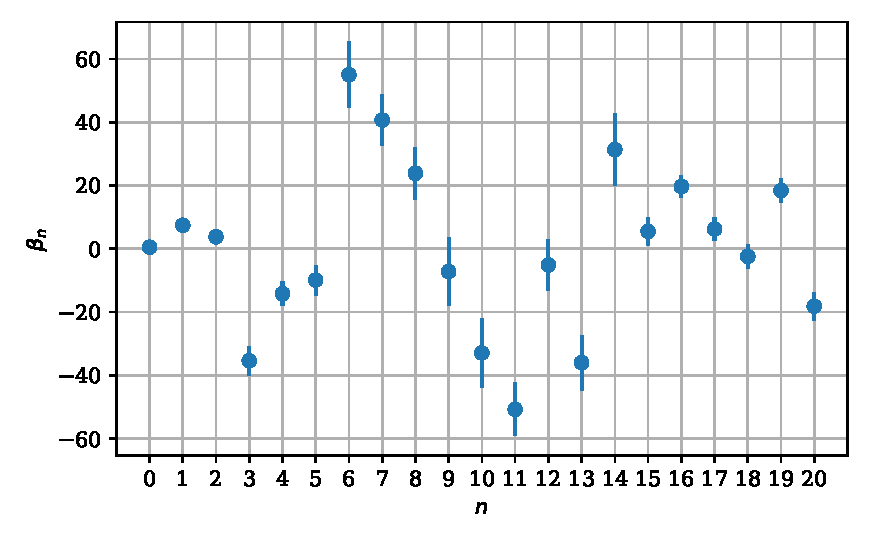
\includegraphics[scale=1]{figs/beta_variance_ols_Franke.pdf}
    \caption{$\bm{\beta}^{\text{OLS}}$  of a fifth order ordinary least squares solution to the Franke function, plotted with $68\%$ confidence intervals.}
    \label{fig:beta_variance_Franke}
\end{figure}

\begin{figure}[H]
    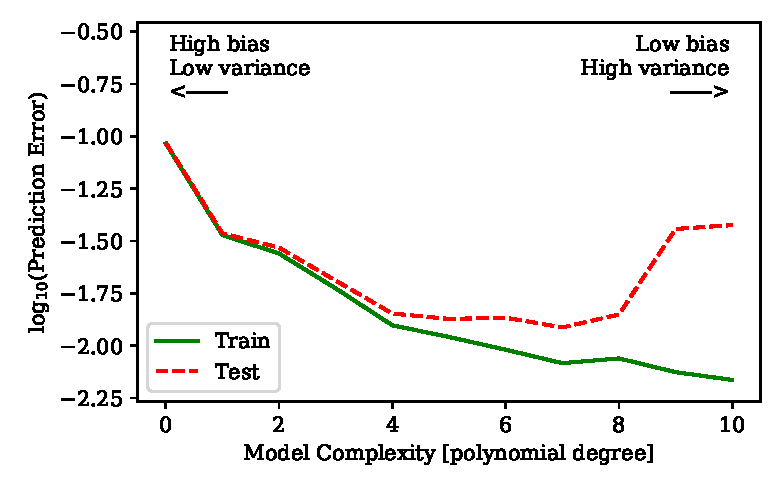
\includegraphics[scale=1]{figs/biasvariancetradeoff_ols_Franke.pdf}
    \caption{Prediction error of training and test set plotted as a function of model complexity (polynomial degree) for the ordinary least squares regression of degree 5 fitted on the Franke's function.}
    \label{fig:bias_ols_Franke}
\end{figure}

\begin{figure}[H]
    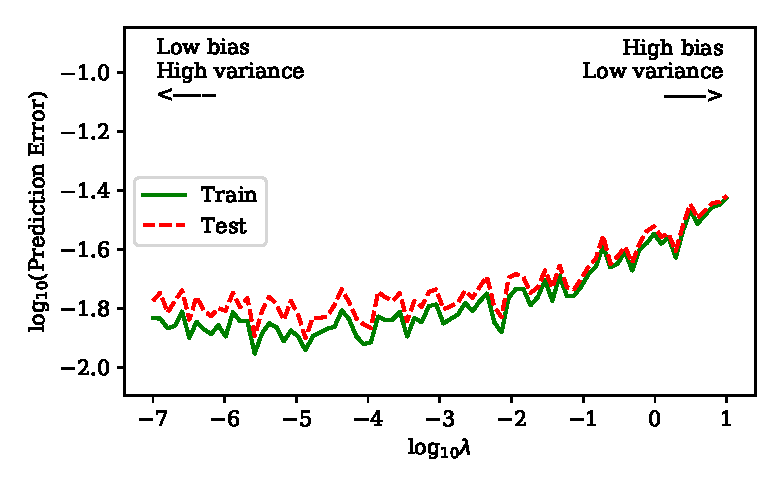
\includegraphics{figs/biasvariancetradeoff_Ridge_Franke.pdf}
    \caption{Prediction error of training and test set plotted as a function of the hyperparameter $\lambda$ for Ridge regression of degree 5 fitted on the Franke's function}
    \label{fig:bias_ridge_Franke}
\end{figure}

\begin{figure}[H]
    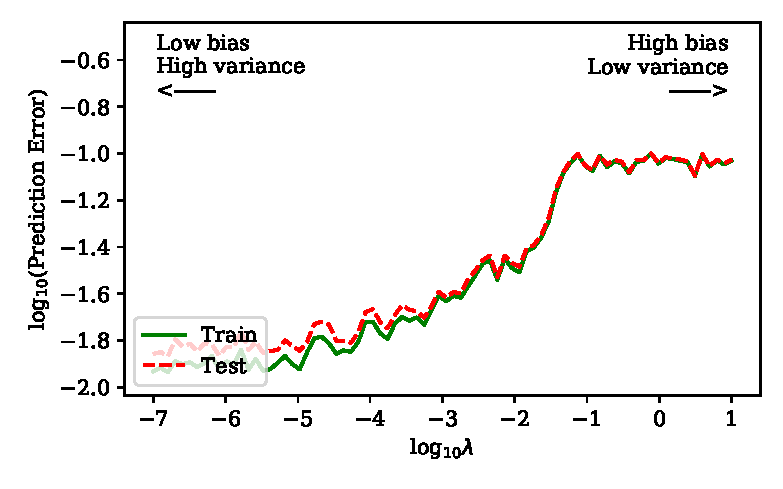
\includegraphics{figs/biasvariancetradeoff_LASSO_Franke.pdf}
    \caption{Prediction error of training and test set plotted as a function of the hyperparameter $\lambda$ for Lasso regression of degree 5 fitted on the Franke's function.}
    \label{fig:bias_lasso_Franke}
\end{figure}
Figures \ref{fig:beta_variance_Franke}, \ref{fig:bias_ridge_Franke} and \ref{fig:bias_lasso_Franke} are all made with a fifth order polynomial fit. This choice was based on the results shown in figure \ref{fig:bias_ols_Franke}, showing the estimated prediction error for varying polynomial degrees.
\subsection{Lake Tanganyika data}

\begin{figure}[H]
    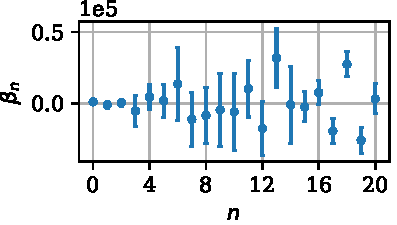
\includegraphics[scale=1]{figs/beta_variance_ols_terrain.pdf}
    \caption{Variance of the beta parameters of a fifth order ordinary least squares fit$\bm{\beta}^{\text{OLS}}$  of a fifth order ordinary least squares fit of terrain data from Lake Tanganyika, Africa, plotted with $68\%$ confidence intervals.}
    \label{fig:beta_variance_terrain}
\end{figure}


\begin{figure}[H]
    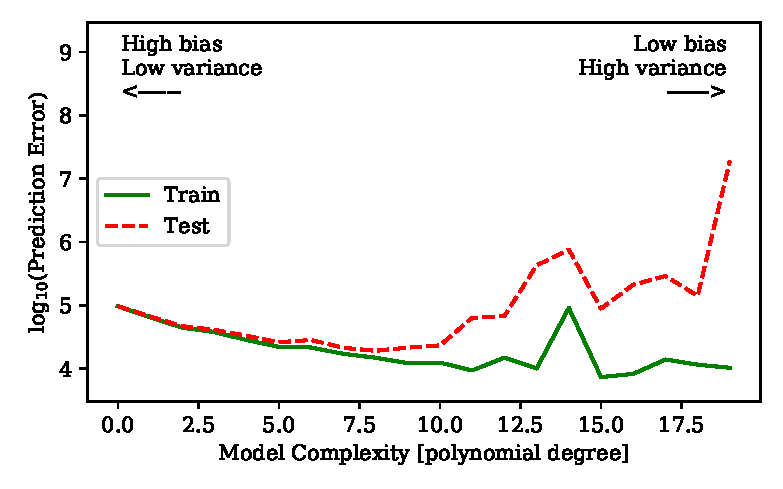
\includegraphics[scale=1]{figs/biasvariancetradeoff_ols_terrain.pdf}
    \caption{Prediction error of training and test set plotted as a function of model complexity (polynomial degree) for the ordinary least squares regression of degree 5 fitted on terrain data of Lake Tanganyika, Africa.}
    \label{fig:bias_ols_terrain}
    
        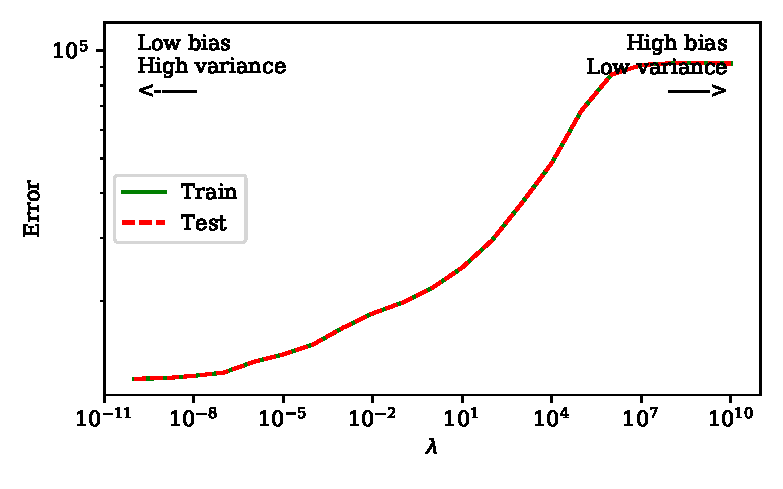
\includegraphics{figs/biasvariancetradeoff_Ridge_terrain.pdf}
    \caption{Prediction error of training and test set plotted as a function of the hyperparameter $\lambda$ for Lasso regression of degree 5 fitted on terrain data of Lake Tanganyika.}

\end{figure}

\begin{figure}[H]
    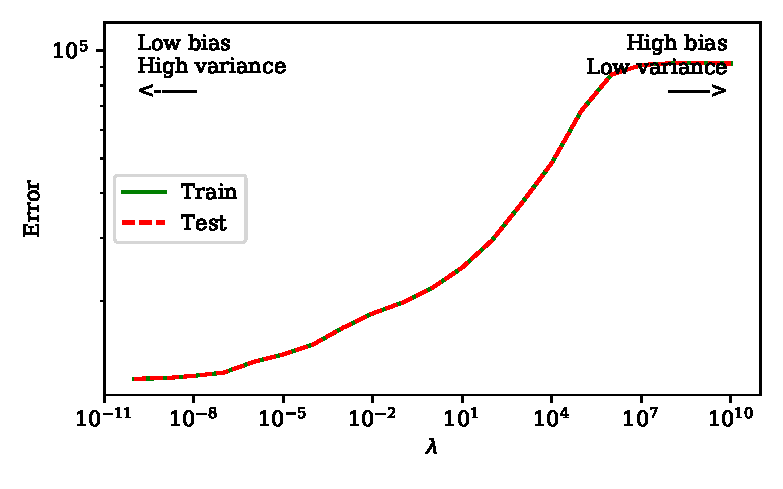
\includegraphics{figs/biasvariancetradeoff_Ridge_terrain.pdf}
    \caption{Prediction error of training and test set plotted as a function of the hyperparameter $\lambda$ for Ridge regression of degree 5 fitted on terrain data of Lake Tanganyika.}
    \label{fig:bias_ridge_terrain}
\end{figure}

\begin{figure}[H]
    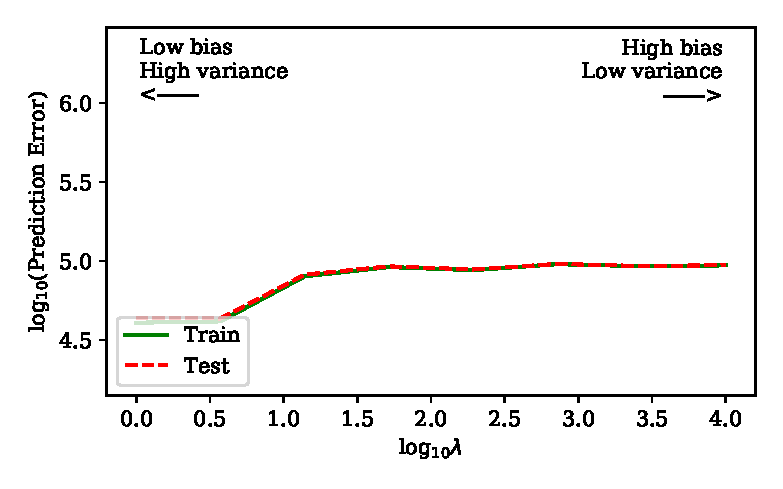
\includegraphics{figs/biasvariancetradeoff_LASSO_terrain.pdf}
    \caption{Prediction error of training and test set plotted as a function of the hyperparameter $\lambda$ for Lasso regression of degree 5 fitted on terrain data of Lake Tanganyika.}
    \label{fig:bias_lasso_terrain}
\end{figure}
As with the results from fitting the Franke's function, figures \ref{fig:beta_variance_terrain}, \ref{fig:bias_ridge_terrain} and \ref{fig:bias_lasso_terrain} are made with a fifth degree polynomial. This choice is based on figure \ref{fig:bias_ols_terrain} and is a compromise between low prediction error and low runtime. In all plots made by analyzing the terrain data from Lake Tanganyika, we only used every 150th point of the data sets to save memory and make the analysis not take too much time to run.
\begin{multicols}{2}





\section{Discussion}
\subsection{Franke's function}

\subsection{Terrain data}

\section{Conclusion}
Duis malesuada sagittis mi ut gravida. Maecenas porta sed mi at malesuada. Nunc et rhoncus nisi, sit amet mattis mauris. Cras lacinia lobortis odio quis ullamcorper. Morbi volutpat turpis est, sit amet efficitur velit viverra ut. Vestibulum eu imperdiet mi. Mauris tincidunt tempor scelerisque. In scelerisque mauris justo, rutrum consectetur tortor cursus in. Vivamus odio diam, interdum eget lobortis ac, vestibulum eu diam. Integer lectus est, pharetra varius ligula et, sodales interdum arcu. Etiam volutpat dolor sit amet justo pharetra, fringilla dictum risus scelerisque.
\end{multicols}



\end{document}
